% Preamble
\documentclass[xcolor=dvipsnames]{beamer}
\usetheme{madrid}

% Packages
\usepackage[english,ngerman]{babel}
\usepackage[utf8]{inputenc}
\usepackage{amsmath}
\usepackage{graphicx}
\usepackage{ifthen} % Boolean variables
\usepackage{subfigure} % Horizontal pictures

\definecolor{hBlue}{RGB}{55,118,165}
\usecolortheme[named=hBlue]{structure}

% Distiction between work and stream presentation
\newboolean{work}
\setboolean{work}{true}

\ifthenelse{\boolean{work}}{
    \titlegraphic{
\includegraphics[width=4cm]{../images/logo.png}}
}{}
\title{Gesundheit \& Ernährung}
\subtitle{Makronährstoffe I: Kohlenhydrate}
\ifthenelse{\boolean{work}}{
    \author{Adrian Helberg}
    \date{16.06.2021}
}{
    \subtitle{twitch.tv/bl1nzlar}
    \author{Bl1nzlar}
    \date{\today}
}


% Document
\begin{document}

    \maketitle

    \frame{\frametitle{Agenda}\tableofcontents}

    \section{Theorie}
    {
    \setbeamercolor{normal text}{fg=hBlue}\usebeamercolor*{normal text}
    \begin{frame}
        \begin{center}
            \Huge Theorie
        \end{center}
    \end{frame}
    }

    \subsection{Profil}
    \begin{frame}
        \frametitle{Profil}

        \begin{block}{Was sind Kohlenhydrate?}
            \begin{itemize}
                \setlength\itemsep{1em}
                \item Grundbaustein der Pflanzen
                \item Kohlenstoffdioxid + Wasser + Sonne (Photosynthese)
                \item Das Kohlenhydrat, dass bei der Photosynthese herauskommt ist der Traubenzucker, als fester, energiereicher Stoff
                \item Unentbehrlich für das Leben auf der Erde
            \end{itemize}
        \end{block}

        \begin{figure}
            \centering
            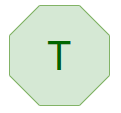
\includegraphics[width=1cm]{../images/t.png}
            \caption{Kohlenhydrat Traubenzucker}
        \end{figure}
    \end{frame}

    \subsection{Traubenzucker}
    \begin{frame}[allowframebreaks]
        \frametitle{Einfachzucker: Traubenzucker}

        \begin{block}{Traubenzucker}
            \begin{itemize}
                \setlength\itemsep{1em}
                \item Alle Lebewesen haben sich um den Traubenzucker als Energiequelle entwickelt
                \item Jede Zelle unseres Körpers kann Traubenzucker zu Energie verbrennen
                \item Traubenzucker lässt sich zu Ketten verbinden
            \end{itemize}
        \end{block}

        \begin{figure}
            \centering
            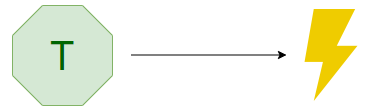
\includegraphics[width=3cm]{../images/t_energie.png}
        \end{figure}

        \framebreak

        \begin{figure}
            \centering
            \subfigure[]{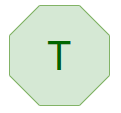
\includegraphics[width=1cm]{../images/t.png}}
            \subfigure[]{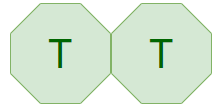
\includegraphics[width=2cm]{../images/t_2.png}}
            \subfigure[]{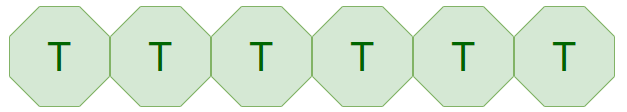
\includegraphics[width=5.4cm]{../images/t_n.png}}
            \caption{(a) Einfachzucker (b) Zweifachzucker (c) Mehrfachzucker}
        \end{figure}

        \framebreak

        \begin{figure}
            \centering
            \subfigure[]{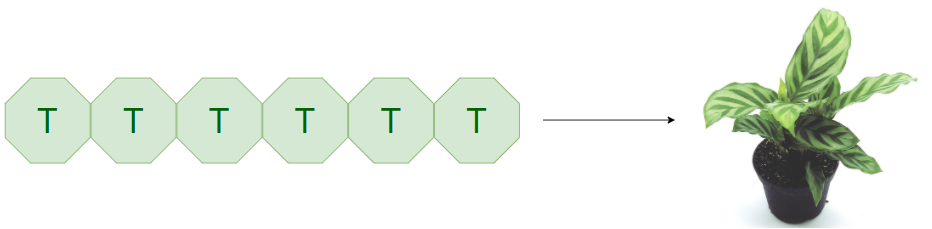
\includegraphics[width=8cm]{../images/pflanzenfasern.png}}
            \subfigure[]{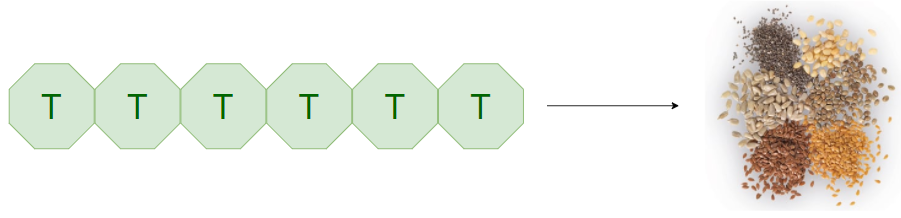
\includegraphics[width=8cm]{../images/samen.png}}
            \caption{(a) Mehrfachzuckerketten als Cellulose ist schwer wieder aufzuspalten und somit schwer verdaulich
                     (b) Pflanzen speichern ihren Mehrfachzucker, der schnell aufgespalten werden soll, zB. in Samen als \textbf{Stärke}}
        \end{figure}

        \framebreak

        \begin{block}{Getreidesamen}
            \begin{itemize}
                \item Weizen, Roggen
                \item Hafer
                \item Reis
                \item Mais
            \end{itemize}
        \end{block}

        \begin{block}{Hülsenfrüchte}
            \begin{itemize}
                \item Bohnen
                \item Linsen
                \item Erbsen
            \end{itemize}
        \end{block}

        \begin{block}{Wurzeln und Knollen}
            \begin{itemize}
                \item Kartoffeln
            \end{itemize}
        \end{block}
    \end{frame}

    \subsection{Fruchtzucker}
    \begin{frame}[allowframebreaks]
        \frametitle{Einfachzucker: Fruchtzucker}

        \begin{block}{Fruchtzucker}
            \begin{itemize}
                \setlength\itemsep{1em}
                \item Kommt in der Natur eher selten vor
                \begin{itemize}
                    \item Reifes Obst
                    \item Bienenhonig
                \end{itemize}
                \item Süßer als Traubenzucker
                \item Fester Bestandteil von Kristallzucker (50\%)
            \end{itemize}
        \end{block}

        \begin{figure}
            \centering
            \subfigure[]{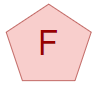
\includegraphics[width=1cm]{../images/F.png}}
            \subfigure[]{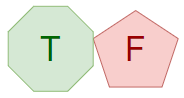
\includegraphics[width=1.8cm]{../images/zucker.png}}
            \caption{(a) Kohlenhydrat Fruchtzucker (b) Haushaltszucker}
        \end{figure}

        \framebreak

        \begin{figure}
            \centering
            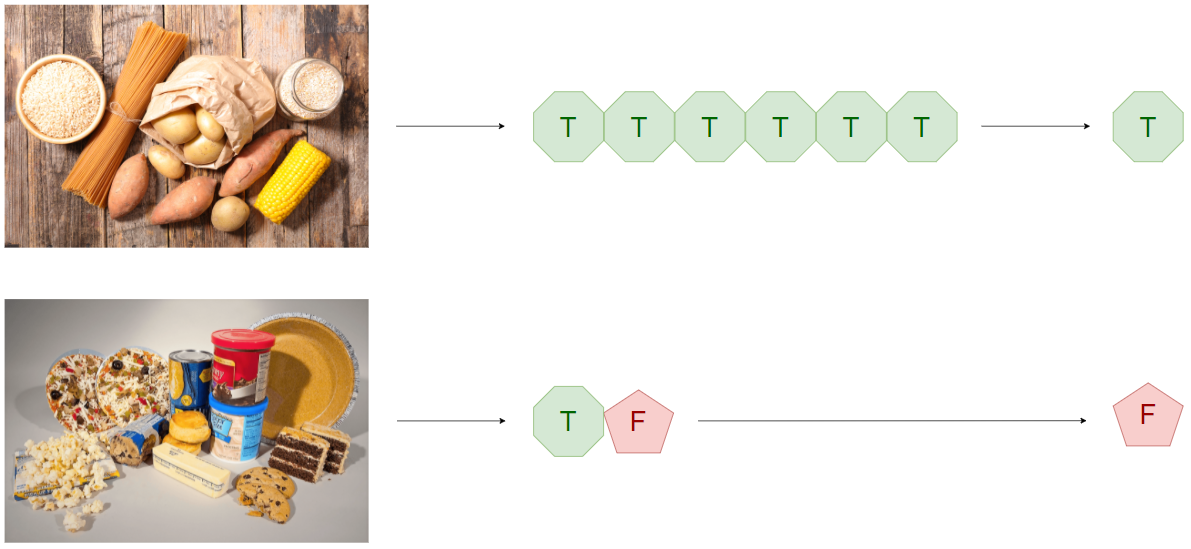
\includegraphics[width=10cm]{../images/t_f.png}
            \caption{Nahrungszucker}
        \end{figure}
    \end{frame}

    \section{Stoffwechsel}
    \begin{frame}[allowframebreaks]
        \frametitle{Stoffwechsel}

        \begin{block}{Traubenzucker}
            \begin{itemize}
                \setlength\itemsep{1em}
                \item Kann von jeder Zelle aufgenommen werden
                \item Kann von jeder Zelle zu Energie verbrannt werden
            \end{itemize}
        \end{block}

        \begin{block}{Fruchtzucker}
            \begin{itemize}
                \setlength\itemsep{1em}
                \item Kann \textbf{nur} von der Leber aufgenommen werden
                \item Muss erst in etwas "`brauchbares"' umgewandelt werden
            \end{itemize}
        \end{block}

        \begin{figure}
            \centering
            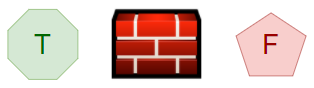
\includegraphics[width=3cm]{../images/wall.png}
            \caption{Traubenzucker und Fruchtzucker sind grundverschieden!}
        \end{figure}

        \framebreak

        \begin{block}{Stärke}
            \begin{itemize}
                \item Makronährstoffe werden im ersten Drittel des Darms aufgenommen
                \item Die Darmwand kann nur Einfachzucker aufnehmen
                \item Aufspaltung in Einfachzucker mithilfe von Verdauungsenzymen
            \end{itemize}
        \end{block}

        \begin{figure}
            \centering
            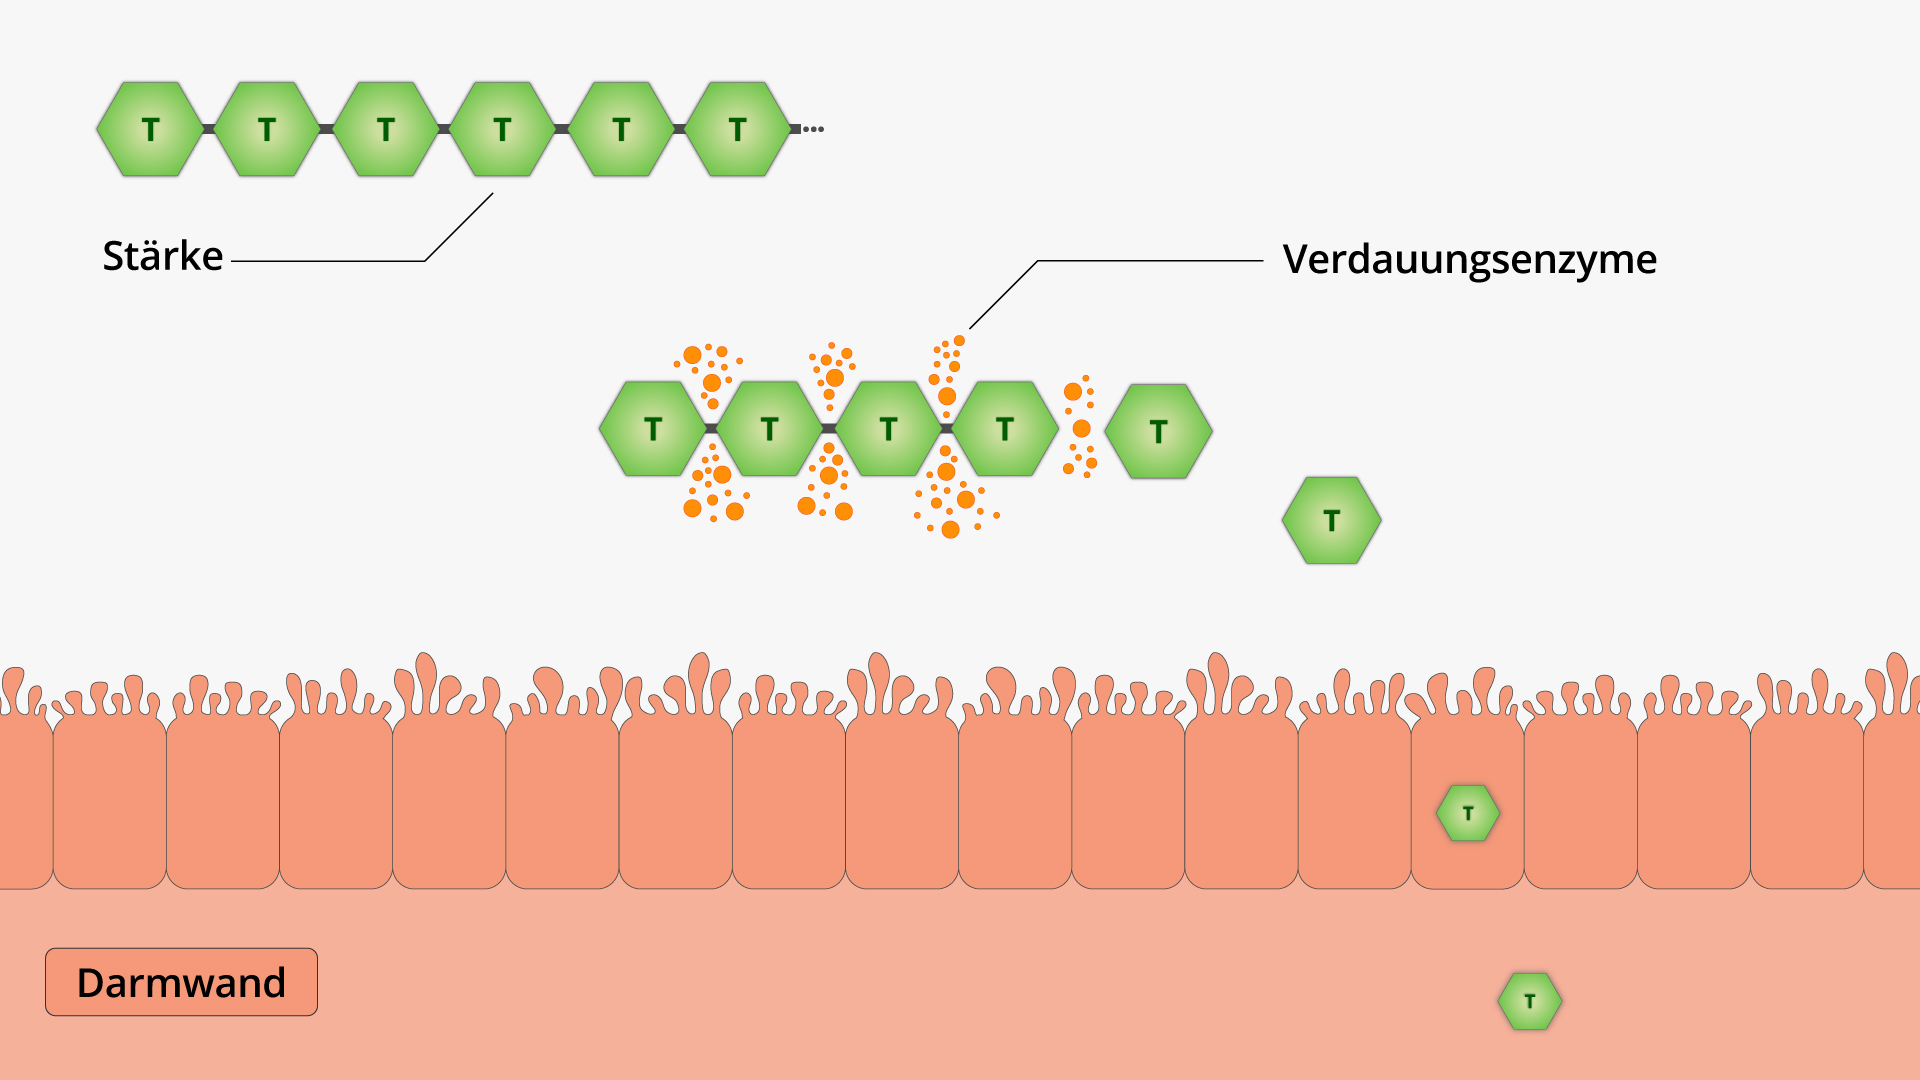
\includegraphics[width=7cm]{../images/verdauung.jpg}
            \caption{Aunahme von Traubenzucker im Dünndarm}
        \end{figure}

        \framebreak

        \begin{figure}
            \centering
            \subfigure[]{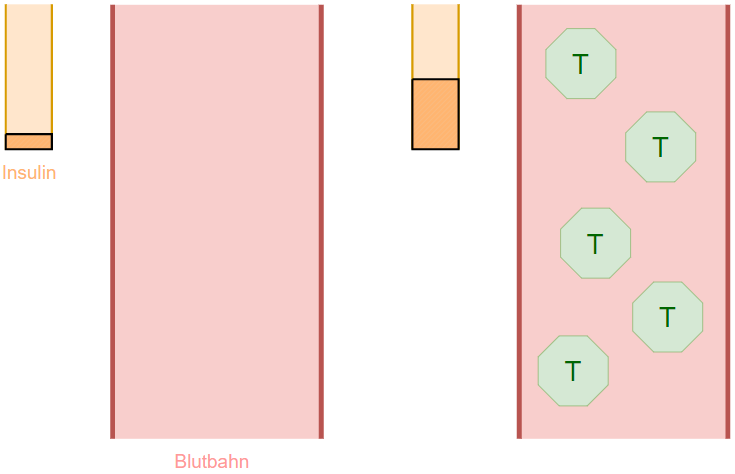
\includegraphics[width=6cm]{../images/blut_1.png}}
            \caption{Anstieg des Blutzuckerspiegels $\rightarrow$ Insulinausschüttung}
        \end{figure}

        \framebreak

        \begin{block}{Insulin}
            \begin{itemize}
                \setlength\itemsep{1em}
                \item Speicher-Hormon
                \item Aufnehmen und Speichern von Nährstoffen (nicht nur Zucker!)
                \item Sorgt nach dem Essen für die Nährstoffaufnahme in Muskeln und Leber
            \end{itemize}
        \end{block}

        \framebreak

        \begin{figure}
            \centering
            \subfigure[]{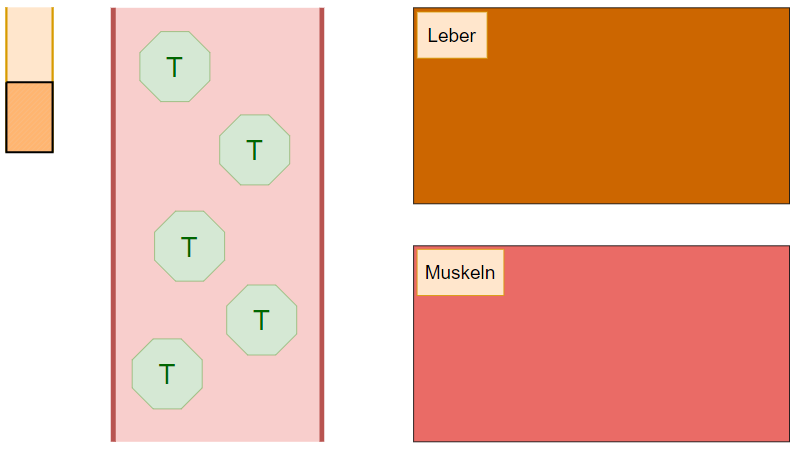
\includegraphics[width=5cm]{../images/blut_2.png}}
            \subfigure[]{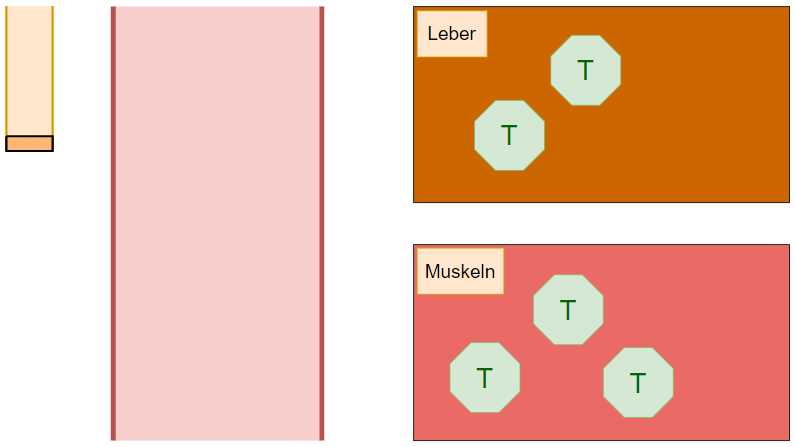
\includegraphics[width=5cm]{../images/blut_3.png}}
            \caption{(a) Hoher und (b) niedriger Blutzuckerspiegel}
        \end{figure}

        \framebreak

        \begin{figure}
            \centering
            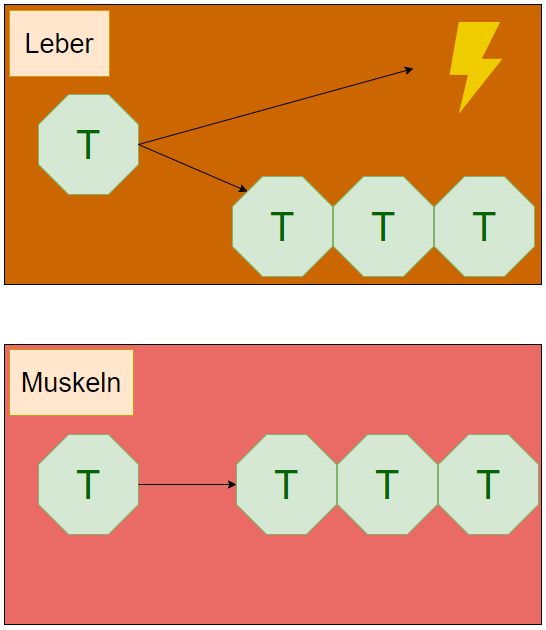
\includegraphics[width=5cm]{../images/leber_1.png}
            \caption{Traubenzucker in Leber und Muskeln}
        \end{figure}

        \framebreak

        \begin{figure}
            \centering
            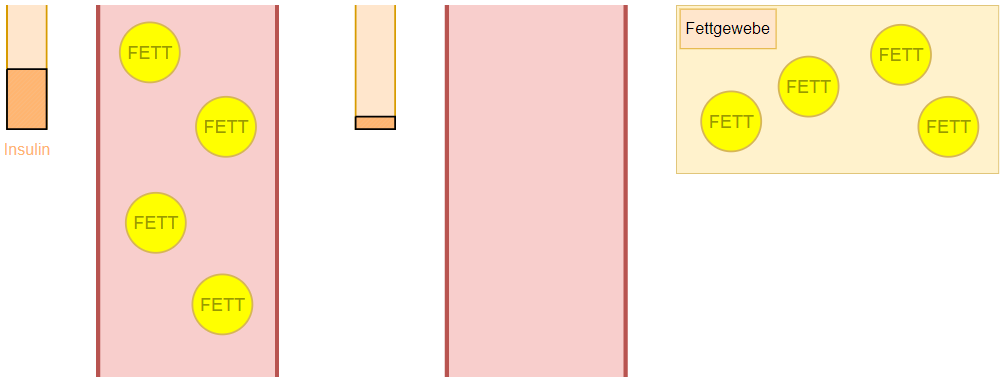
\includegraphics[width=10cm]{../images/fettgewebe.png}
            \caption{Auswirkung Insulin auf Fett}
        \end{figure}

        \framebreak

        \begin{figure}
            \centering
            \subfigure[]{\includegraphics[width=2cm]{../images/nüchtern.png}}
            \subfigure[]{\includegraphics[width=2cm]{../images/nüchtern_1.png}}
            \subfigure[]{\includegraphics[width=2cm]{../images/nüchtern_2.png}}
            \subfigure[]{\includegraphics[width=2cm]{../images/nüchtern_3.png}}
            \caption{(a) Insulinspiegel verdauend (b) Insulinspiegel nüchtern (c) gestörter Insulinspiegel nüchtern (d) gestörter Insulinspiegel verdauend}
        \end{figure}

        \framebreak

        \begin{block}{Gestörter Insulinhaushalt}
            \begin{itemize}
                \setlength\itemsep{1em}
                \item Bei chronisch hohem Insulinspiegel, ist der Fettstoffwechsel zugunsten des Fettaufbaus verlagert
            \end{itemize}
        \end{block}

    \end{frame}

    \section{Praxis}
    {
        \setbeamercolor{normal text}{fg=hBlue}\usebeamercolor*{normal text}
        \begin{frame}
            \begin{center}
                \Huge Praxis
            \end{center}
        \end{frame}
    }

    \section{Fragerunde}
    {
        \setbeamercolor{normal text}{fg=hBlue}\usebeamercolor*{normal text}
        \begin{frame}
            \begin{center}
                \Huge Fragerunde
            \end{center}
        \end{frame}
    }

\end{document}